\documentclass[11pt,a4paper]{report}
\usepackage[spanish,es-nodecimaldot]{babel}
\usepackage{fontspec}
\setmainfont{Arial}
\setsansfont{Arial}
\usepackage{geometry}
\geometry{margin=2.4cm}
\usepackage{graphicx}
\usepackage{booktabs,longtable,tabularx,array,pdflscape}
\usepackage{amsmath}
\usepackage{xcolor}
\usepackage{listings}
\usepackage{fancyhdr}
\usepackage[numbers,sort&compress]{natbib}
\usepackage{xurl}
\usepackage[hidelinks]{hyperref}
\usepackage[capitalise,noabbrev]{cleveref}
\definecolor{igpblue}{HTML}{176B87}
\definecolor{igpgreen}{HTML}{4C956C}
\definecolor{codegray}{HTML}{F2F4F4}
\hypersetup{pdftitle={SPOTPY como herramienta de experimentación, sensibilidad y calibración para modelos hidrológicos},pdfauthor={Jhon Gesell Villanueva Portella}}
\lstset{basicstyle=\ttfamily\small,backgroundcolor=\color{codegray},frame=single,breaklines=true,columns=fullflexible,keepspaces=true}
\pagestyle{fancy}\fancyhf{}\lhead{SPOTPY Laboratory for SWAT+ IGP}\rhead{PP00089}\cfoot{\thepage}
\setlength{\headheight}{14pt}
\setcounter{tocdepth}{2}
\begin{document}
\begin{titlepage}
\centering
\vspace*{1.7cm}
{\color{igpblue}\rule{\textwidth}{2pt}}\\[1.2cm]
{\Huge\bfseries SPOTPY como herramienta de experimentación, sensibilidad y calibración para modelos hidrológicos:\par}
\vspace{0.5cm}{\LARGE laboratorio reproducible orientado a SWAT+ IGP\par}
\vspace{1.2cm}{\Large Proyecto PP00089 - Instituto Geofísico del Perú\par}
\vfill
{\large Autor editable: Jhon Gesell Villanueva Portella\par}
\vspace{0.3cm}{\large Versión del laboratorio: SPOTPY 1.6.7\par}
\vspace{0.3cm}{\large \today\par}
\vspace{1.2cm}{\color{igpgreen}\rule{\textwidth}{2pt}}
\end{titlepage}
\chapter*{Resumen ejecutivo}\addcontentsline{toc}{chapter}{Resumen ejecutivo}
Este manual documenta un laboratorio ejecutado y verificable, no sólo una propuesta. Explica qué recibe SPOTPY, cómo envuelve un modelo, qué persiste y cómo se interpretan exploración, sensibilidad, calibración, multiobjetivo e incertidumbre. MC, LHS, FAST, SCE-UA y DDS están probados; las capacidades avanzadas se clasifican con cautela. La conexión con SWAT+ se presenta como arquitectura futura: no se afirma una integración real sin ejecutable, proyecto, parámetros, unidades y parser verificados.
\tableofcontents
\listoffigures
\listoftables
\chapter{Introducción}
SPOTPY es una biblioteca Python para estimar, explorar y analizar parámetros de modelos mediante algoritmos intercambiables \citep{houska2015spotpy}. Resuelve el problema operativo de conectar un modelo arbitrario con muestreo, optimización, sensibilidad o incertidumbre sin reescribir el algoritmo para cada modelo.

No limpia precipitación, corrige temperatura, procesa DEM, delimita cuencas, genera HRU ni construye proyectos SWAT+. Esas tareas pertenecen al preprocesamiento. SPOTPY empieza cuando existe un contrato reproducible que transforma parámetros y forzantes en una simulación comparable con observaciones.

Un parámetro calibrable es una entrada incierta expuesta al sampler mediante nombre, distribución prior y límites. Una iteración es una evaluación de un conjunto: se ejecuta el modelo, se obtiene una serie y se calcula un objetivo. El sampler genera conjuntos, objetivos, simulaciones y, según el método, cadenas o índices de sensibilidad. La calibración busca buen ajuste en un período; la validación comprueba capacidad fuera de ese período sin reajustar. La incertidumbre describe distribuciones plausibles, no sólo un óptimo.

El laboratorio usa un modelo lluvia-caudal didáctico de 30 pasos. Por ello demuestra operatividad, no validez hidrológica para una cuenca peruana.


\chapter{Arquitectura de SPOTPY}
Una clase setup implementa cuatro puntos de integración:
\begin{description}
\item[\texttt{parameters()}] declara priors, límites y nombres y entrega candidatos al algoritmo.
\item[\texttt{simulation(vector)}] aplica el vector al modelo y devuelve la serie simulada.
\item[\texttt{evaluation()}] entrega observaciones alineadas en longitud y orden.
\item[\texttt{objectivefunction(simulation,evaluation)}] reduce la comparación a un escalar o vector de objetivos.
\end{description}

El sampler llama repetidamente ese contrato y su base de datos añade prefijos \texttt{like*}, \texttt{par*}, \texttt{simulation\_*} y \texttt{chain}. El mejor candidato se determina respetando la orientación real: máximo para scores como NSE en DDS; mínimo para la pérdida interna de SCE-UA.

\begin{figure}[htbp]\centering
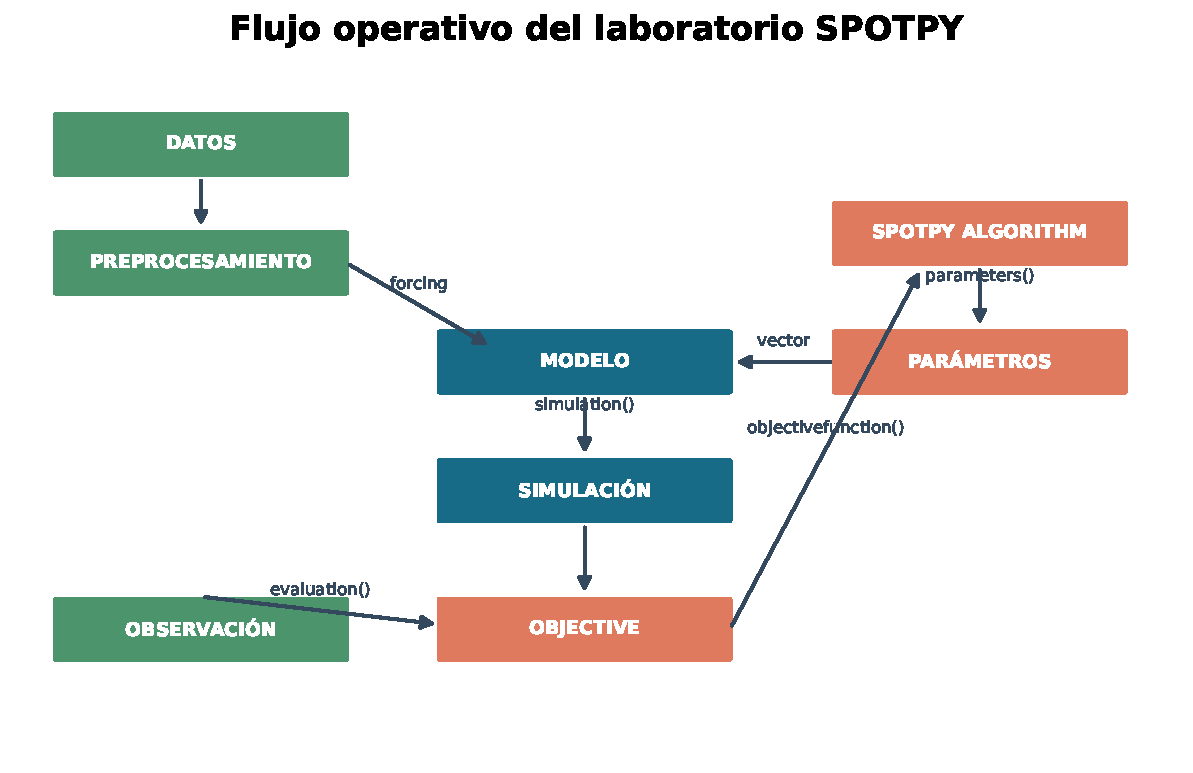
\includegraphics[width=\textwidth]{figures/spotpy_workflow.pdf}
\caption{Flujo ejecutado por el setup y el sampler.}\label{fig:workflow}
\end{figure}

La figura~\ref{fig:workflow} separa el preprocesamiento de SPOTPY. La flecha de retorno representa la decisión del algoritmo sobre el siguiente conjunto.

\chapter{Entorno verificado}
Se creó un entorno Conda aislado; no se modificó \texttt{base} ni Python global.
\begin{table}[htbp]\centering\caption{Versiones ejecutadas.}\label{tab:versions}
\begin{tabular}{ll}\toprule Componente & Versión\\\midrule
Python & 3.12.13\\ SPOTPY & 1.6.7\\ NumPy & 2.5.2\\ SciPy & 1.18.0\\ Pandas & 3.0.5\\ Matplotlib & 3.11.1\\ pytest & 9.1.1\\\bottomrule
\end{tabular}\end{table}

La instalación no incluye \texttt{mpi4py}, PyTables/HDF5, \texttt{pathos} ni \texttt{multiprocess}. La ejecución validada es secuencial. \texttt{environment.yml} y \texttt{requirements.txt} fijan las versiones. \texttt{pip check} no reporta requisitos rotos.


\chapter{Entradas, procesos y salidas}
El input hidrológico concreto se encuentra en
\path{03_hydrology_demo/data/input.csv}. Contiene \texttt{date},
\texttt{precip\_mm}, \texttt{pet\_mm} y \texttt{q\_obs}. Las dos variables climáticas están nombradas en mm; el código no define si son acumulados o promedios. La unidad de caudal no está definida: no debe presentarse como m³/s.

El lector rechaza archivo ausente, columnas faltantes, NaN, fechas inválidas, duplicadas o desordenadas, valores no numéricos y negativos. La tabla completa de campos y validaciones está en \path{docs/07_input_process_output.md}.

\begin{landscape}
\scriptsize
\begin{longtable}{p{2.1cm}p{3.0cm}p{2.0cm}p{2.0cm}p{3.6cm}p{3.0cm}p{2.2cm}p{2.0cm}}
\caption{Tabla maestra de entradas, procesos y salidas.}\label{tab:masterio}\\
\toprule Etapa & Entrada concreta & Formato & Unidad & Proceso & Salida concreta & Formato & Unidad\\\midrule\endfirsthead
\toprule Etapa & Entrada concreta & Formato & Unidad & Proceso & Salida concreta & Formato & Unidad\\\midrule\endhead
Clima & \texttt{date, precip\_mm, pet\_mm} & CSV & fecha, mm, mm & Validación Pandas & forcing & DataFrame & mismas\\
Observación & \texttt{q\_obs} & CSV float & no definida & validación/alineamiento & evaluation & array & no definida\\
Modelo & forcing + 5 parámetros & arrays & mixta & balances de reservorios & \texttt{q\_sim} & array & no definida\\
Parámetros & rangos Uniform & objetos & mixta & \texttt{parameters()} & candidato & ParameterSet & mixta\\
Simulación & candidato + forcing & Python & mixta & \texttt{simulation()} & serie & array & no definida\\
Evaluación & \texttt{q\_obs} & DataFrame & no definida & \texttt{evaluation()} & referencia & array & no definida\\
Objetivo & sim + obs & arrays & no definida & \texttt{objectivefunction()} & score/loss & float/list & [-], \%, o Q\\
Sampling & setup, runs, seed & CLI/config & n/a & \texttt{sample()} & evaluaciones & CSV/RAM/SQL & mixta\\
FAST & 325 candidatos & diseño FAST & parámetros & Fourier & S1/ST & CSV/PNG & [-]\\
SCE-UA & 120 nominales & sampler & n/a & complejos; minimiza -NSE & calibrado & CSV/JSON/PNG & mixta\\
DDS & 120 & sampler & n/a & dimensiones dinámicas; maximiza NSE & calibrado & CSV/JSON/PNG & mixta\\
Externo & JSON + input CSV & archivos & mixta & subprocess + timeout & \texttt{output.csv} & CSV & no definida\\
Futuro SWAT+ & copia + parámetros verificados & por definir & por definir & \texttt{swatplus.exe} & Q simulada & por verificar & objetivo futuro: m³/s\\
\bottomrule
\end{longtable}
\end{landscape}



Cada run conserva configuración, entorno, registro, base SPOTPY, métricas, parámetros, serie inicial/mejor y figuras. Los archivos centrales son \texttt{config.json}, \texttt{environment.json}, \texttt{run.log} y \texttt{metrics.json}. Las columnas \texttt{simulation\_0...29} no incluyen fecha; el índice temporal se recupera del input validado.

\chapter{Rosenbrock: contrato mínimo}
Rosenbrock separa la mecánica SPOTPY de la hidrología. Los parámetros son $x\in[-2,2]$ e $y\in[-1,3]$ y la pérdida es
\[f(x,y)=(1-x)^2+100(y-x^2)^2.\]
El óptimo global es $(1,1)$ con $f=0$. En 100 muestras MC y semilla 42, el laboratorio obtuvo $f=0.188121$, $x=0.763751$, $y=0.546941$. No alcanzar exactamente el óptimo con un presupuesto corto es esperable. El ejemplo enseña base CSV, selección por mínimo y trazabilidad sin confundir resultados con una simulación física.


\chapter{Modelo hidrológico didáctico}
El modelo contiene reservorios de suelo, respuesta rápida y base. Precipitación y PET impulsan 30 pasos diarios. Sus parámetros se listan en \cref{tab:parameters}.
\begin{table}[htbp]\centering\small\caption{Parámetros didácticos; no son parámetros SWAT+.}\label{tab:parameters}
\begin{tabular}{lrrll}\toprule Parámetro & Mín. & Máx. & Prior & Unidad\\\midrule
runoff\_coeff & 0.05&0.85&Uniform&[-]\\ soil\_capacity&20&250&Uniform&mm, por consistencia interna\\ et\_factor&0.2&1.5&Uniform&[-]\\ quick\_recession&0.15&0.95&Uniform&fracción/paso\\ base\_recession&0.005&0.25&Uniform&fracción/paso\\\bottomrule
\end{tabular}\end{table}

MC con 50 muestras produjo NSE 0.908542 y KGE 0.898044. Estos valores verifican que el pipeline puede recuperar un buen candidato respecto del conjunto sintético; no validan estructura, unidades ni capacidad predictiva en otra época. Una calibración científica necesita warm-up, separación calibración/validación, incertidumbre observacional y datos suficientemente largos.


\chapter{Funciones objetivo y métricas}
Con observado $O_i$ y simulado $S_i$, NSE es
\[\mathrm{NSE}=1-\frac{\sum_i(S_i-O_i)^2}{\sum_i(O_i-\bar O)^2}.\]
Su ideal es 1 y se maximiza. KGE combina correlación, razón de variabilidad y razón de medias; su ideal también es 1 \citep{gupta2009kge}. RMSE y MAE conservan la unidad desconocida del caudal y se minimizan. PBIAS se expresa en porcentaje; en este laboratorio positivo significa sobreestimación. $R^2$ mide asociación, no ausencia de sesgo.

SCE-UA está configurado por SPOTPY 1.6.7 para minimizar; por ello recibe $-\mathrm{NSE}$. DDS maximiza y recibe NSE natural. Los JSON vuelven a calcular las métricas con signo hidrológico natural. Esta separación evita elegir accidentalmente el peor candidato.

Una likelihood no es automáticamente una métrica. Para DREAM se usó una
likelihood gaussiana con error de medición, no NSE. Su nombre en la API es
\begin{lstlisting}
gaussianLikelihoodMeasErrorOut
\end{lstlisting}
La validez bayesiana depende de un modelo explícito y defendible del error.

\chapter{Sensibilidad FAST y eFAST}
Sensibilidad pregunta cuánto cambia un output al variar inputs; calibración busca valores que ajustan observaciones. FAST asigna frecuencias a parámetros y descompone varianza mediante Fourier \citep{cukier1973fast}. Con 325 evaluaciones, el ranking ST fue: runoff\_coeff 0.88951; quick\_recession 0.39920; base\_recession 0.04214; soil\_capacity 0.03988; et\_factor 0.02907.

Un ST alto significa influencia dentro de estos rangos, este modelo y esta métrica; no prueba causalidad universal ni identifica el mejor valor. Antes de SWAT+ ayuda a reducir/priorizar parámetros si sus rangos son defendibles.

eFAST extiende el diseño para estimar contribuciones espectrales \citep{saltelli1999efast}. SPOTPY exigió 71 corridas para cinco parámetros y devolvió fracciones parciales: 0.3138 para runoff\_coeff y 0.1293 para quick\_recession, las dos mayores. El mínimo exacto demuestra ejecución, no estabilidad comparativa con FAST.


\chapter{Calibración: SCE-UA y DDS}
SCE-UA evoluciona complejos para afrontar óptimos múltiples en modelos lluvia-caudal \citep{duan1992sceua}. Se solicitaron 120 evaluaciones; SPOTPY realizó 225 internas y guardó 88. El mejor interno alcanzó NSE 0.954195, KGE 0.860940, RMSE 0.657595 y PBIAS -8.996\%. El análisis usa el estado interno porque el CSV omitió candidatos descartados por la evolución.

DDS reduce dinámicamente el número de dimensiones perturbadas conforme avanza el presupuesto \citep{tolson2007dds}. Con 120 evaluaciones obtuvo NSE 0.963318, KGE 0.981289, RMSE 0.588474 y PBIAS 0.292\%.

DDS resultó mejor en este caso, semilla y presupuesto; no demuestra superioridad universal. Validación significaría congelar parámetros y evaluar otro período, tarea pendiente por longitud del dataset.


\chapter{Control de un modelo externo}
El adaptador ficticio materializa el puente hacia un solver: crea directorio UUID, escribe parámetros, lanza un proceso con \texttt{subprocess.run}, fija \texttt{cwd}/timeout, captura stdout/stderr, verifica return code y archivo, parsea \texttt{output.csv} y limpia o preserva.

Los tests cubren éxito, fallo y timeout. Una ejecución fallida genera una excepción con causa; no debe contaminar otros workers. SPOTPY sólo necesita que \texttt{simulation()} traduzca el conjunto candidato a esa secuencia y devuelva la serie.

La demostración usa Python como ejecutable externo. Sustituirlo por \texttt{swatplus.exe} requiere verificar archivos, parámetros, unidades y salida real; no basta cambiar el nombre del comando.


\chapter{Arquitectura futura SWAT+ IGP}
\begin{figure}[htbp]\centering
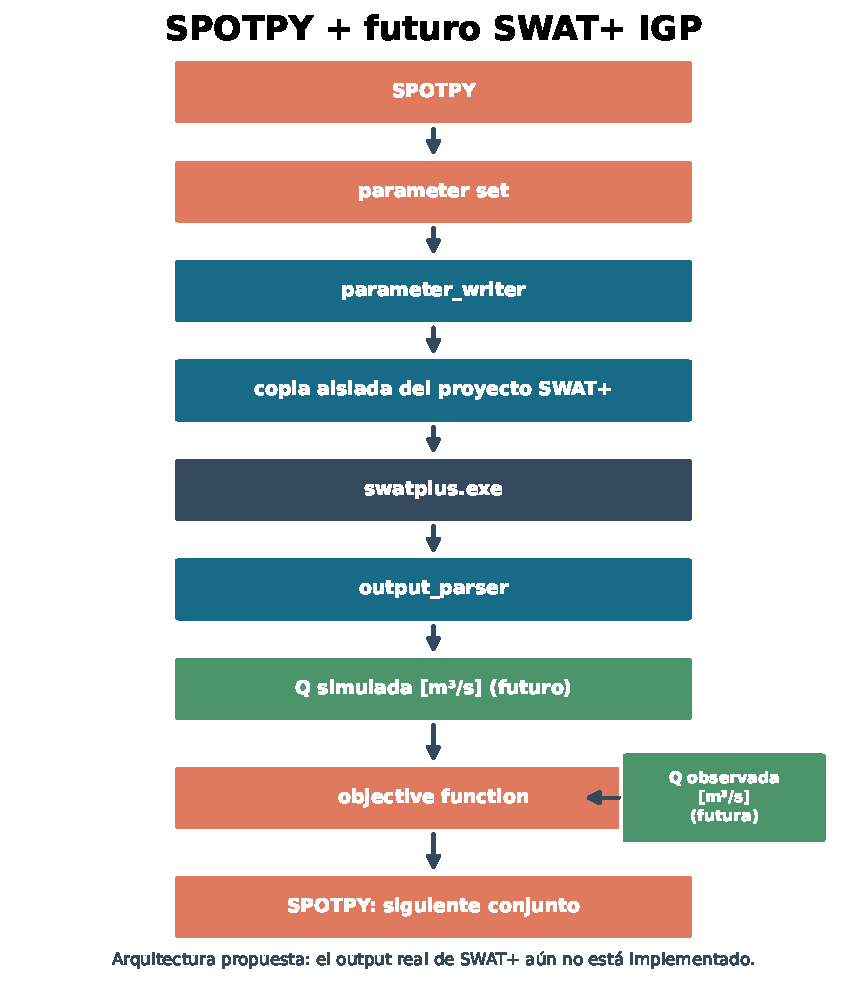
\includegraphics[width=.92\textwidth,height=.78\textheight,keepaspectratio]{figures/spotpy_swatplus_workflow.pdf}
\caption{Arquitectura propuesta; no representa una ejecución SWAT+ ya implementada.}\label{fig:swat}
\end{figure}

Faltan para integración real: ejecutable/version exacta; copia controlada del proyecto; parámetros, archivos y semántica de modificación; archivo/columna de caudal; unidades; estación y calendario; warm-up; reinicio; baseline; manejo de fallos y concurrencia. La Q futura se desea en m³/s, pero el laboratorio actual no define la unidad de \texttt{q\_obs}.

Cada worker debe poseer una copia mutable independiente. Compartir un proyecto produce carreras, outputs mezclados y corrupción. Se debe verificar primero una sola corrida secuencial y su reproducibilidad bit a bit o dentro de tolerancia documentada.

\chapter{Capacidades avanzadas evaluadas}
\section{Firmas hidrológicas}
Sobre 30 días se calcularon media (4.1473), Q5 (9.585), Q50 (3.1), Q95 (0.6585), coeficiente de variación (0.7409), razón media/mediana (1.3378), autocorrelación lag-1 (0.0804) y 0\% de ceros. Las firmas con dimensión de Q conservan unidad desconocida. No se forzaron frecuencias anualizadas, extremos anuales, recesión ni baseflow.

\section{NSGA-II}
NSGA-II conserva diversidad por dominancia y crowding \citep{deb2002nsgaii}. Se minimizaron por separado $1-$NSE, $1-$KGE y $|$PBIAS$|/100$. Se guardaron 48 evaluaciones y 8 filas no dominadas. Un frente de Pareto describe trade-offs; no produce un ganador sin preferencias. La ejecución emitió un warning numérico de crowding por rango objetivo nulo en un subconjunto; terminó y generó evidencia, pero el presupuesto es sólo didáctico. PA-DDS continúa marcado beta en la fuente instalada.

\section{DREAM y posterior}
DREAM evoluciona múltiples cadenas mediante diferencias adaptativas \citep{vrugt2009dream}. Con siete cadenas y 140 registros, los R-hat finales estuvieron entre 2.07 y 4.47, muy por encima del criterio 1.2: \textbf{no convergió}. El diagnóstico se relaciona con la comparación entre/ dentro de cadenas \citep{gelman1992diagnostic}. El top 20\% por likelihood es demostrativo y no se presenta como posterior robusta. DE-MCz y Geweke quedan no probados.

\section{Bases}
RAM, CSV y SQLite conservaron 20 registros idénticamente muestreados. RAM es efímera; CSV transparente; SQLite consultable. En Windows, SQL exige \texttt{dbname} relativo porque SPOTPY lo reutiliza como nombre de tabla. HDF5 no se probó por ausencia de PyTables.


\chapter{Reproducibilidad}
Desde Anaconda Prompt:
\begin{lstlisting}[language=bash]
cd C:\Users\ACER\Documents\GitHub\spotpy_tests
conda activate spotpy-igp
python 01_smoke_test\run_smoke_test.py
python run_experiment.py --example rosenbrock --algorithm mc --runs 100
python 03_hydrology_demo\run_demo.py
python run_experiment.py --example hydrology --algorithm lhs --runs 100
python run_experiment.py --example hydrology --algorithm fast --runs 325
python run_experiment.py --example hydrology --algorithm sceua --runs 500
python run_experiment.py --example hydrology --algorithm dds --runs 500
python 08_external_model_adapter\run_demo.py
python -m pytest -v
\end{lstlisting}

Los experimentos avanzados se ejecutan mediante los scripts \path{run_signatures.py},
\path{run_nsga2.py}, \path{run_dream.py}, \path{run_efast.py} y
\path{run_backends.py}, cada uno desde su directorio numerado.

Para recompilar este documento desde la raíz:
\begin{lstlisting}[language=bash]
cd latex
xelatex -interaction=nonstopmode -halt-on-error -jobname=SPOTPY_IGP_Manual main.tex
bibtex SPOTPY_IGP_Manual
xelatex -interaction=nonstopmode -halt-on-error -jobname=SPOTPY_IGP_Manual main.tex
xelatex -interaction=nonstopmode -halt-on-error -jobname=SPOTPY_IGP_Manual main.tex
\end{lstlisting}
La semilla 42 está fijada donde la API lo permite. Cada ejecución normal crea identificador con microsegundos y no sobrescribe runs anteriores.

\chapter{Conclusiones}
El laboratorio prueba que SPOTPY puede separar modelo, datos, objetivos y algoritmos, persistir experimentos y controlar procesos externos. FAST, SCE-UA y DDS ya aportan un camino claro hacia sensibilidad y calibración alrededor de SWAT+.

La principal brecha no es añadir más samplers. Es definir científicamente inputs/units, verificar un proyecto SWAT+, separar calibración/validación, adoptar una likelihood defendible y garantizar directorios por worker. DREAM demostró correctamente una no-convergencia; NSGA-II demostró el contrato multiobjetivo sin declarar un frente estable.

El próximo paso recomendado es una única corrida SWAT+ reproducible sobre copia controlada, con writer/parser testeados y Q observada/simulada realmente expresada en m³/s. Sólo después corresponde aumentar evaluaciones o paralelizar.


\bibliographystyle{plainnat}
\bibliography{references}
\end{document}
